% Drawing lattice points and vectors
% Author: Bill Tourloupis
\documentclass{article}
\usepackage{tikz}
\usetikzlibrary{calc}
\begin{document}
\begin{figure}[ht]
  \centering
  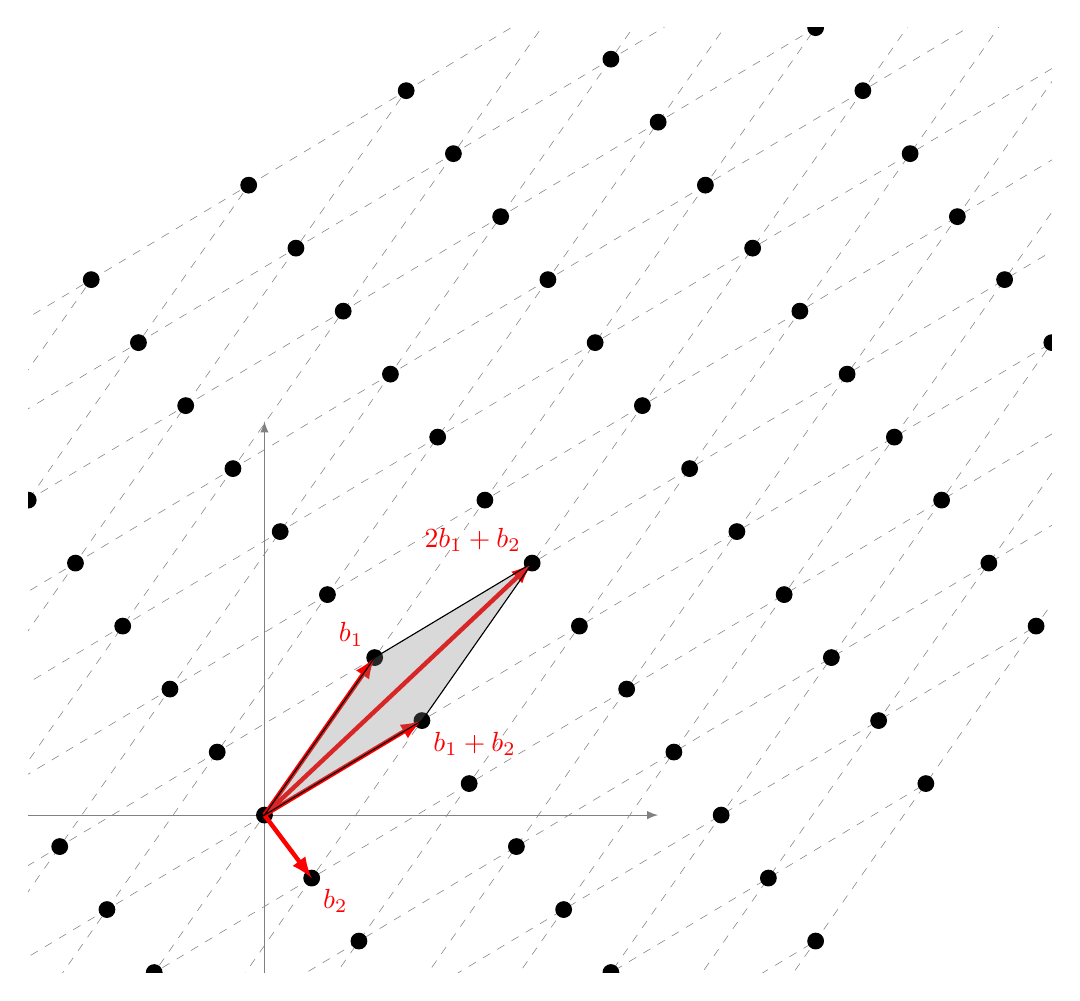
\begin{tikzpicture}
    \coordinate (Origin)   at (0,0);
    \coordinate (XAxisMin) at (-3,0);
    \coordinate (XAxisMax) at (5,0);
    \coordinate (YAxisMin) at (0,-2);
    \coordinate (YAxisMax) at (0,5);
    \draw [thin, gray,-latex] (XAxisMin) -- (XAxisMax);% Draw x axis
    \draw [thin, gray,-latex] (YAxisMin) -- (YAxisMax);% Draw y axis

    \clip (-3,-2) rectangle (10cm,10cm); % Clips the picture...
    \pgftransformcm{1}{0.6}{0.7}{1}{\pgfpoint{0cm}{0cm}}
          % This is actually the transformation matrix entries that
          % gives the slanted unit vectors. You might check it on
           % MATLAB etc. . I got it by guessing.
    \coordinate (Bone) at (0,2);
    \coordinate (Btwo) at (2,-2);
    \draw[style=help lines,dashed] (-14,-14) grid[step=2cm] (14,14);
          % Draws a grid in the new coordinates.
          %\filldraw[fill=gray, fill opacity=0.3, draw=black] (0,0) rectangle (2,2);
              % Puts the shaded rectangle
    \foreach \x in {-7,-6,...,7}{% Two indices running over each
      \foreach \y in {-7,-6,...,7}{% node on the grid we have drawn 
        \node[draw,circle,inner sep=2pt,fill] at (2*\x,2*\y) {};
            % Places a dot at those points
      }
    }
    \draw [ultra thick,-latex,red] (Origin)
        -- (Bone) node [above left] {$b_1$};
    \draw [ultra thick,-latex,red] (Origin)
        -- (Btwo) node [below right] {$b_2$};
    \draw [ultra thick,-latex,red] (Origin)
        -- ($(Bone)+(Btwo)$) node [below right] {$b_1+b_2$};
    \draw [ultra thick,-latex,red] (Origin)
        -- ($2*(Bone)+(Btwo)$) node [above left] {2$b_1+b_2$};
    \filldraw[fill=gray, fill opacity=0.3, draw=black] (Origin)
        rectangle ($2*(Bone)+(Btwo)$);
    %\draw [thin,-latex,red, fill=gray, fill opacity=0.3] (0,0)
        % -- ($2*(0,2)+(2,-2)$)
        % -- ($3*(0,2)+2*(2,-2)$) -- ($(0,2)+(2,-2)$) -- cycle;
  \end{tikzpicture}
  \caption{Babai's algorithm works poorly if the basis is ``bad''.}
  \label{figure:solving-CVP-bad-basis}
\end{figure}
\end{document}
